\chapter{Supplementary Material}

\begin{figure}[H]
	\centering
	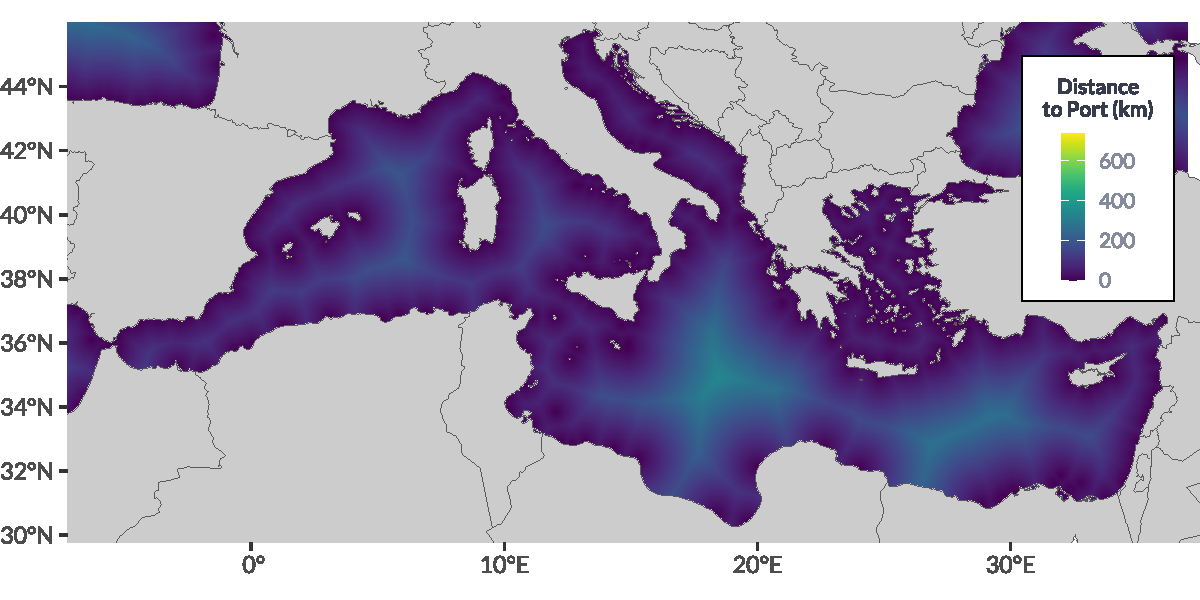
\includegraphics[width=1\linewidth, trim=0 0 0 0,clip]{Figures/plots/dist_med.pdf}
	\caption{Distance to port in km throughout the Mediterranean. }
	\label{fig:distance}
\end{figure}

\begin{figure}[H]
	\centering
	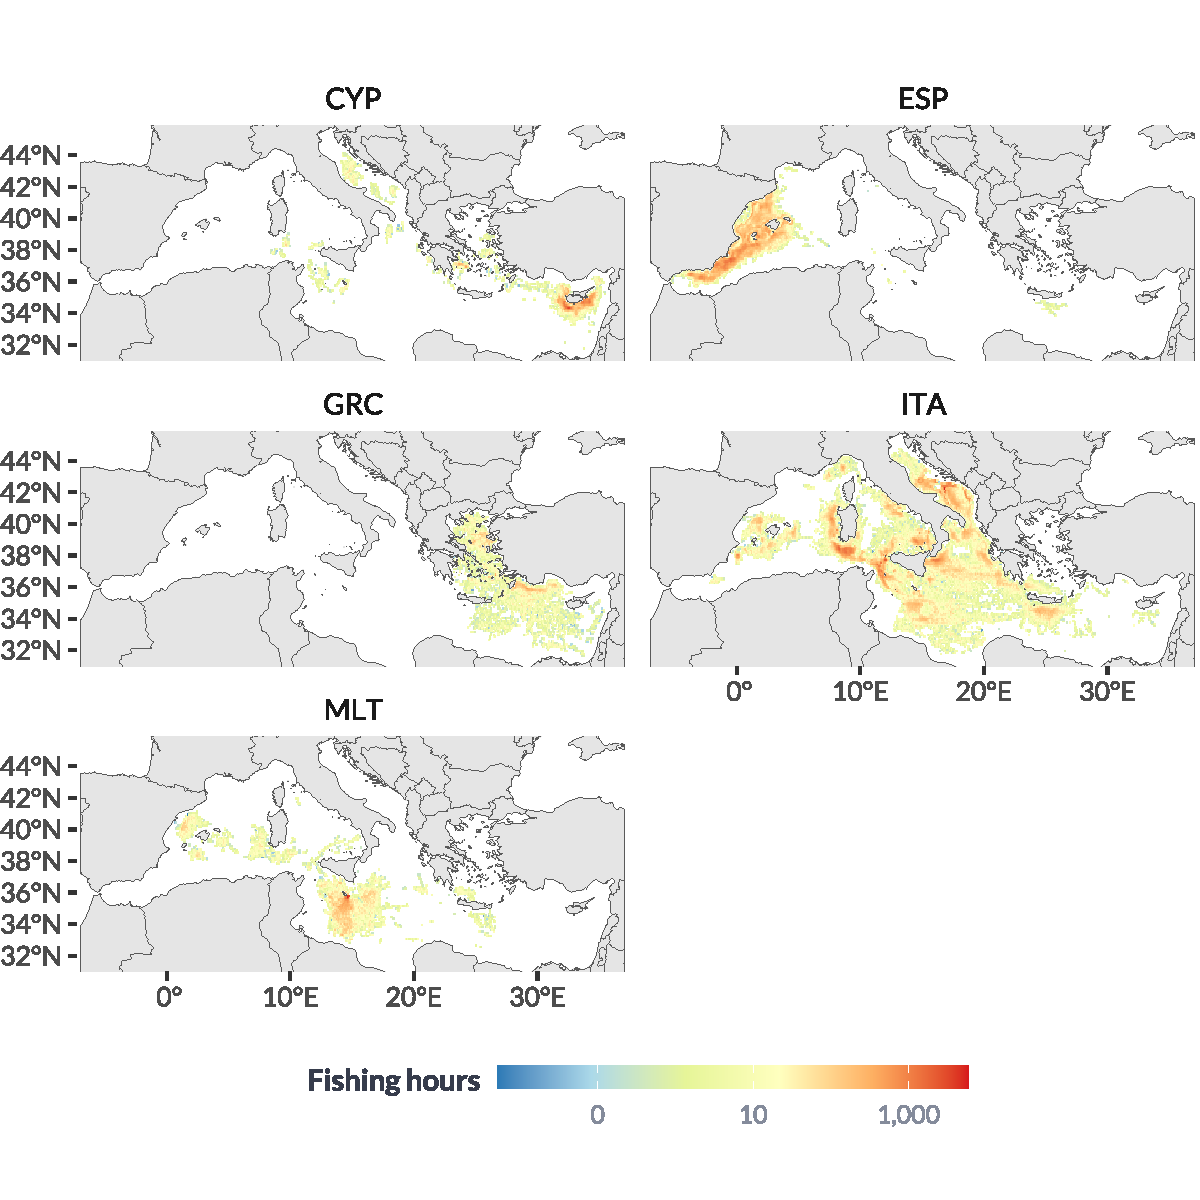
\includegraphics[width=1\linewidth, trim=0 1.2cm 0 1.2cm,clip]{Figures/plots/longline_countries.pdf}
	\caption{Sum of longline fishing hours per flag country (2015-2024). CYP = Cyprus; ESP = Spain, GRC = Greece, ITA = Italy, MLT = Malta}
	\label{fig:longline_effort_countries}
\end{figure}

\begin{figure}[H]
	\centering
	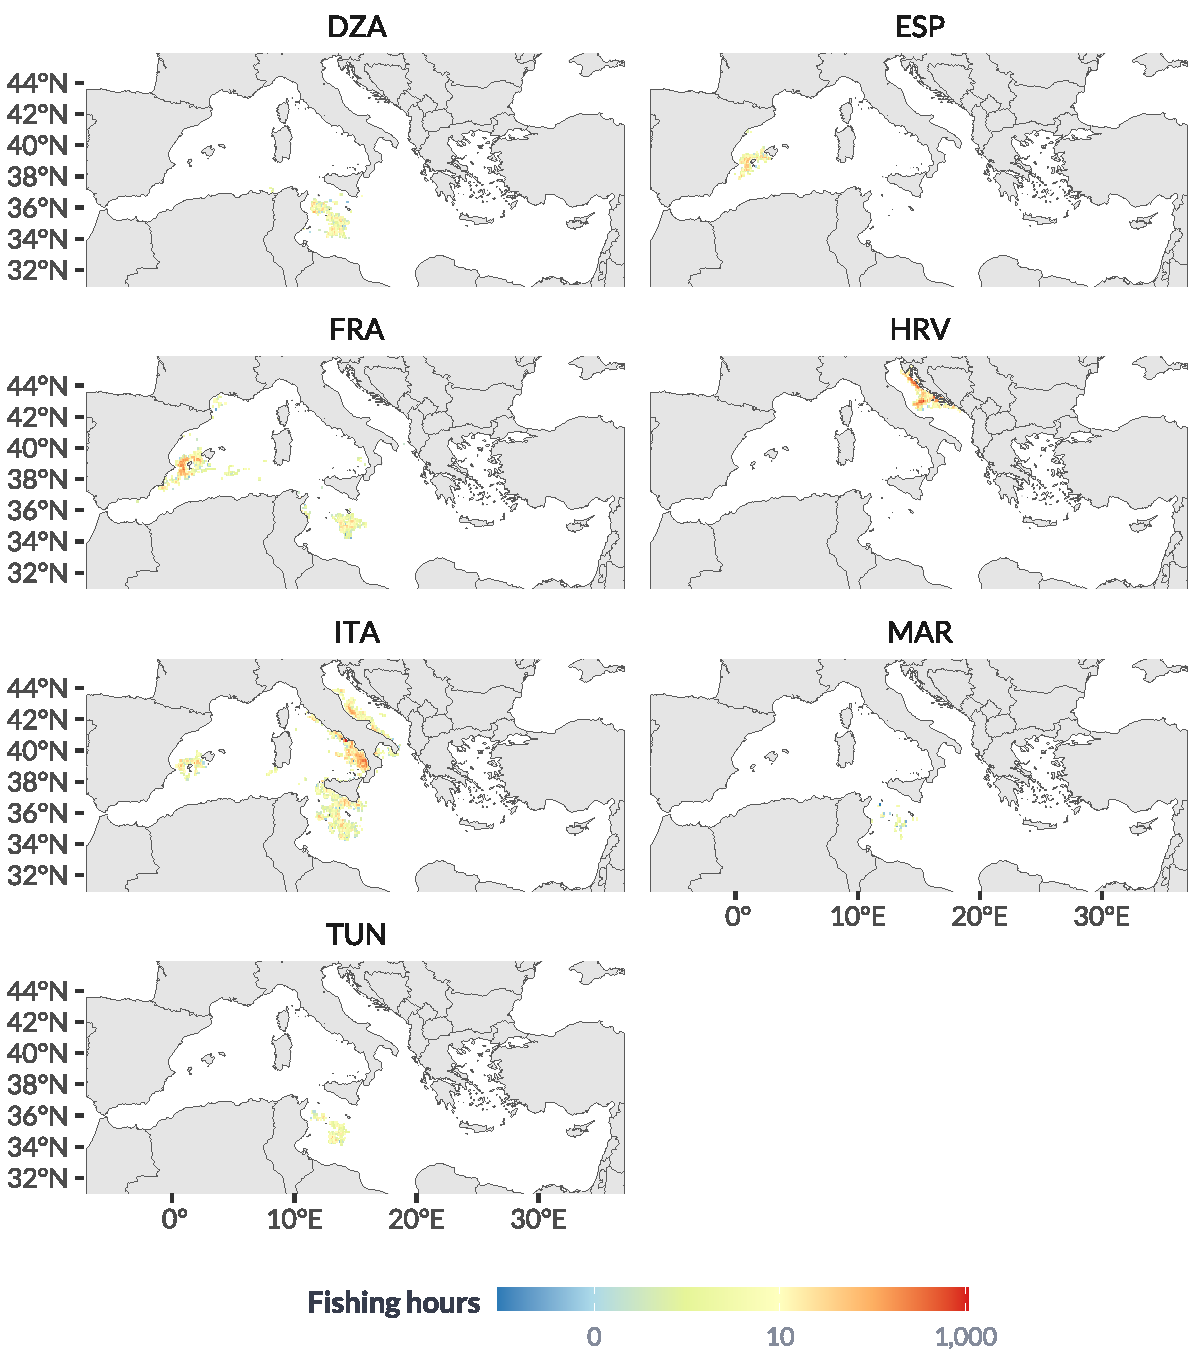
\includegraphics[width=1\linewidth, trim=0 0 0 0,clip]{Figures/plots/seines_countries.pdf}
	\caption{Sum of purse seine fishing hours per flag country (2015-2024). DZA = Algeria, ESP = Spain, FRA = France,
		HRV = Croatia, ITA = Italy, MAR = Morocco, TUN = Tunisia.}
	\label{fig:seine_effort_countries}
\end{figure}

\begin{figure}[H]
	\centering
	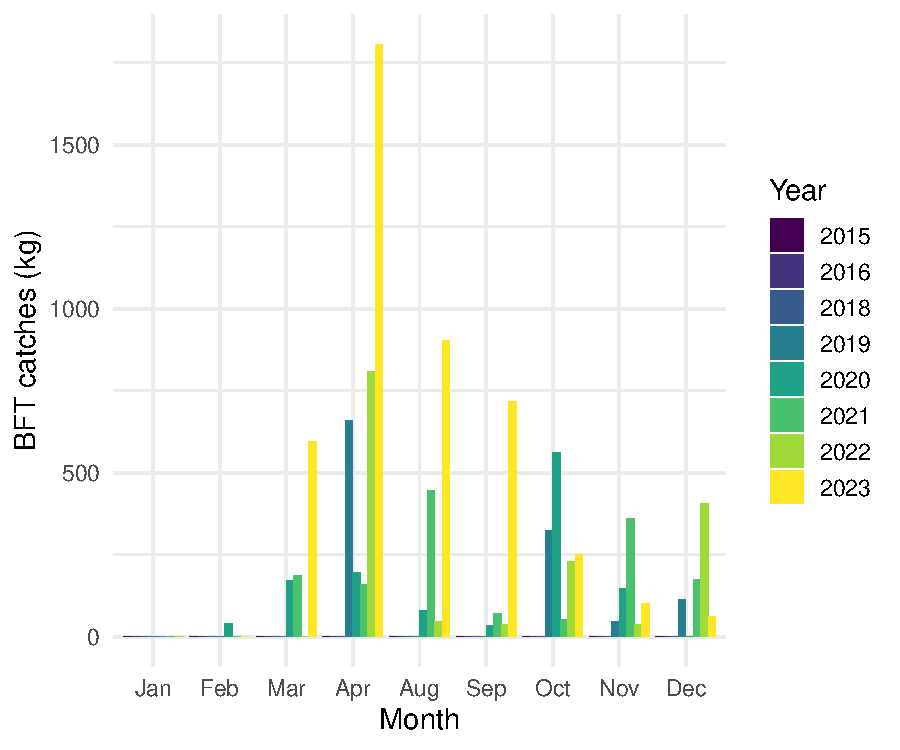
\includegraphics[width=1\linewidth, trim=0 0 0 0,clip]{Figures/plots/hrv_catches.pdf}
	\caption{Reported bluefin tuna (BFT) purse seine catches of Croatia. May, June, and July were excluded as they are orders of magnitude higher and did not
		allow for graphic comparison between months with lower activity.}
	\label{fig:hrv}
\end{figure}

%\begin{figure}[H]
%	\centering
%	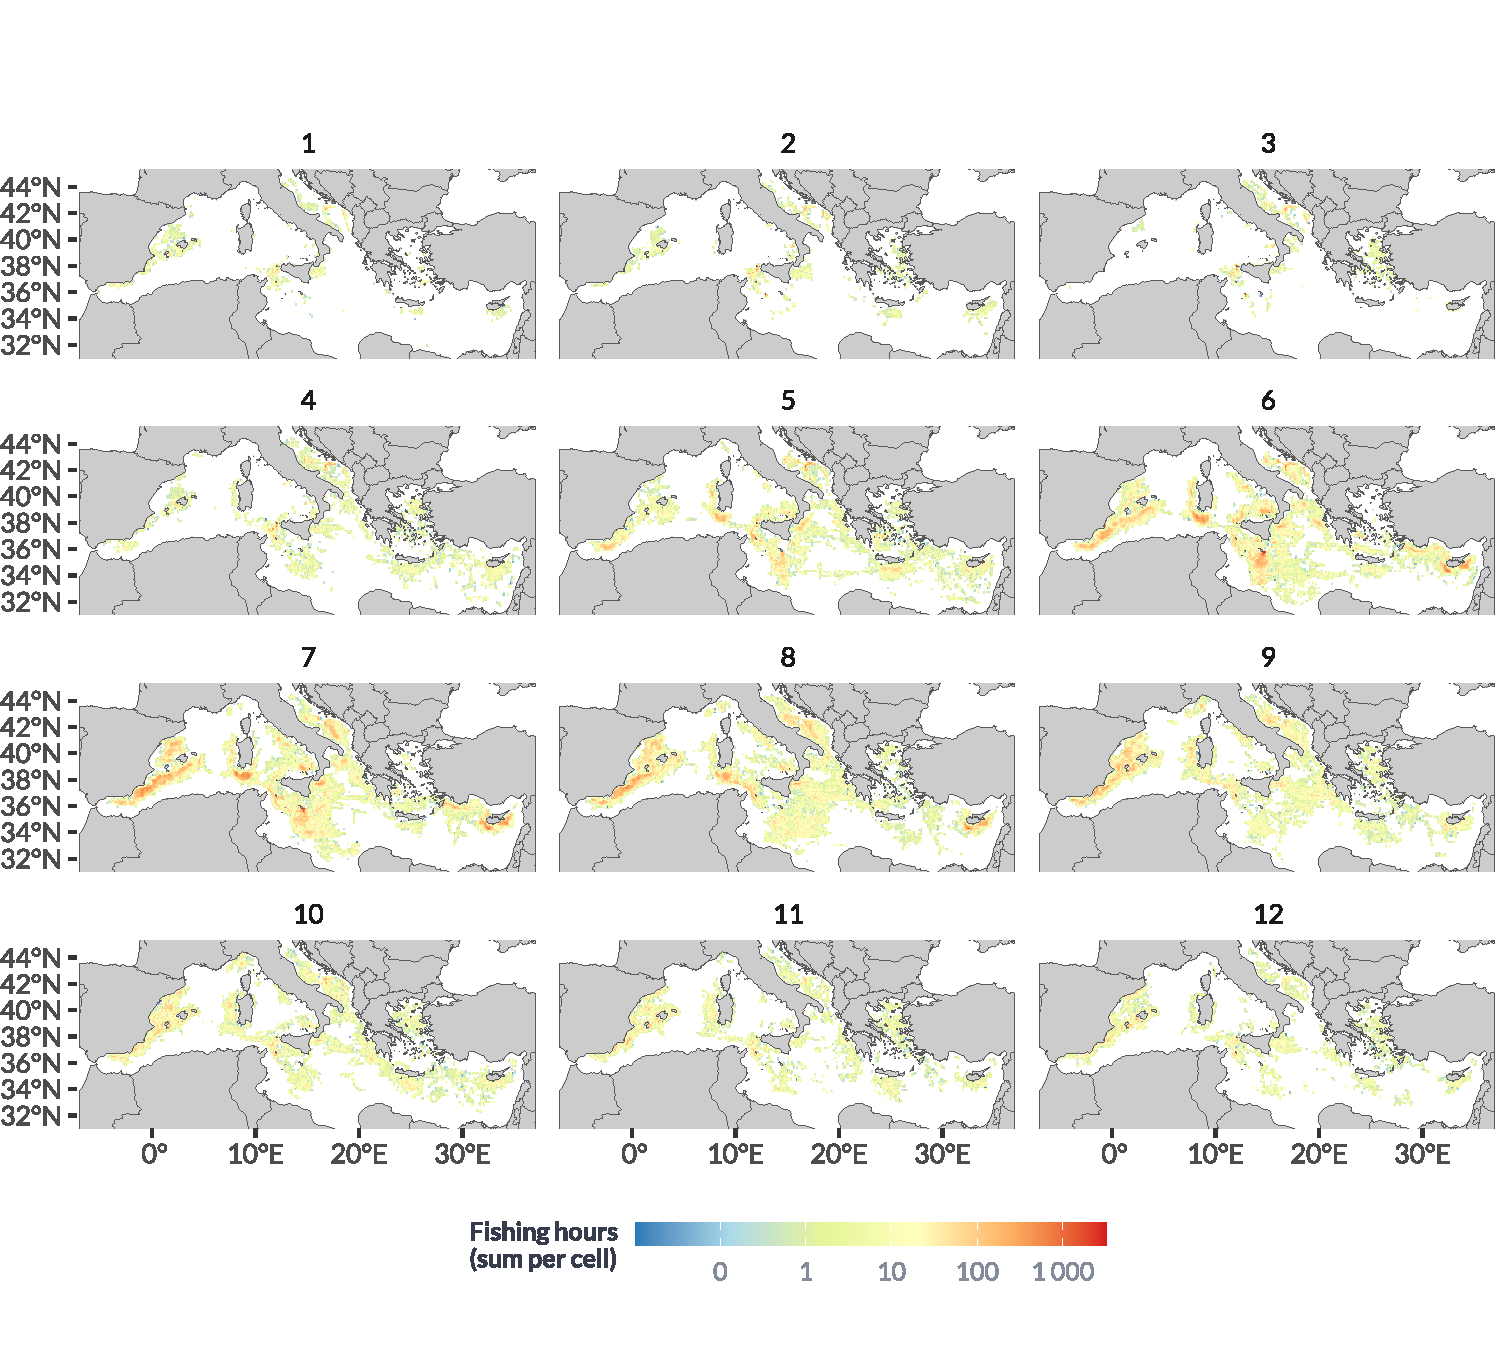
\includegraphics[width=1\linewidth, trim=0 1cm 0 1cm,clip]{Figures/plots/dll_monthly.pdf}
%	\caption{Sum of longline fishing hours per cell for each month between 2015-2024. Colours are on a log-scale.}
%	\label{fig:dll_monthly}
%\end{figure}

%\begin{figure}[H]
%	\centering
%	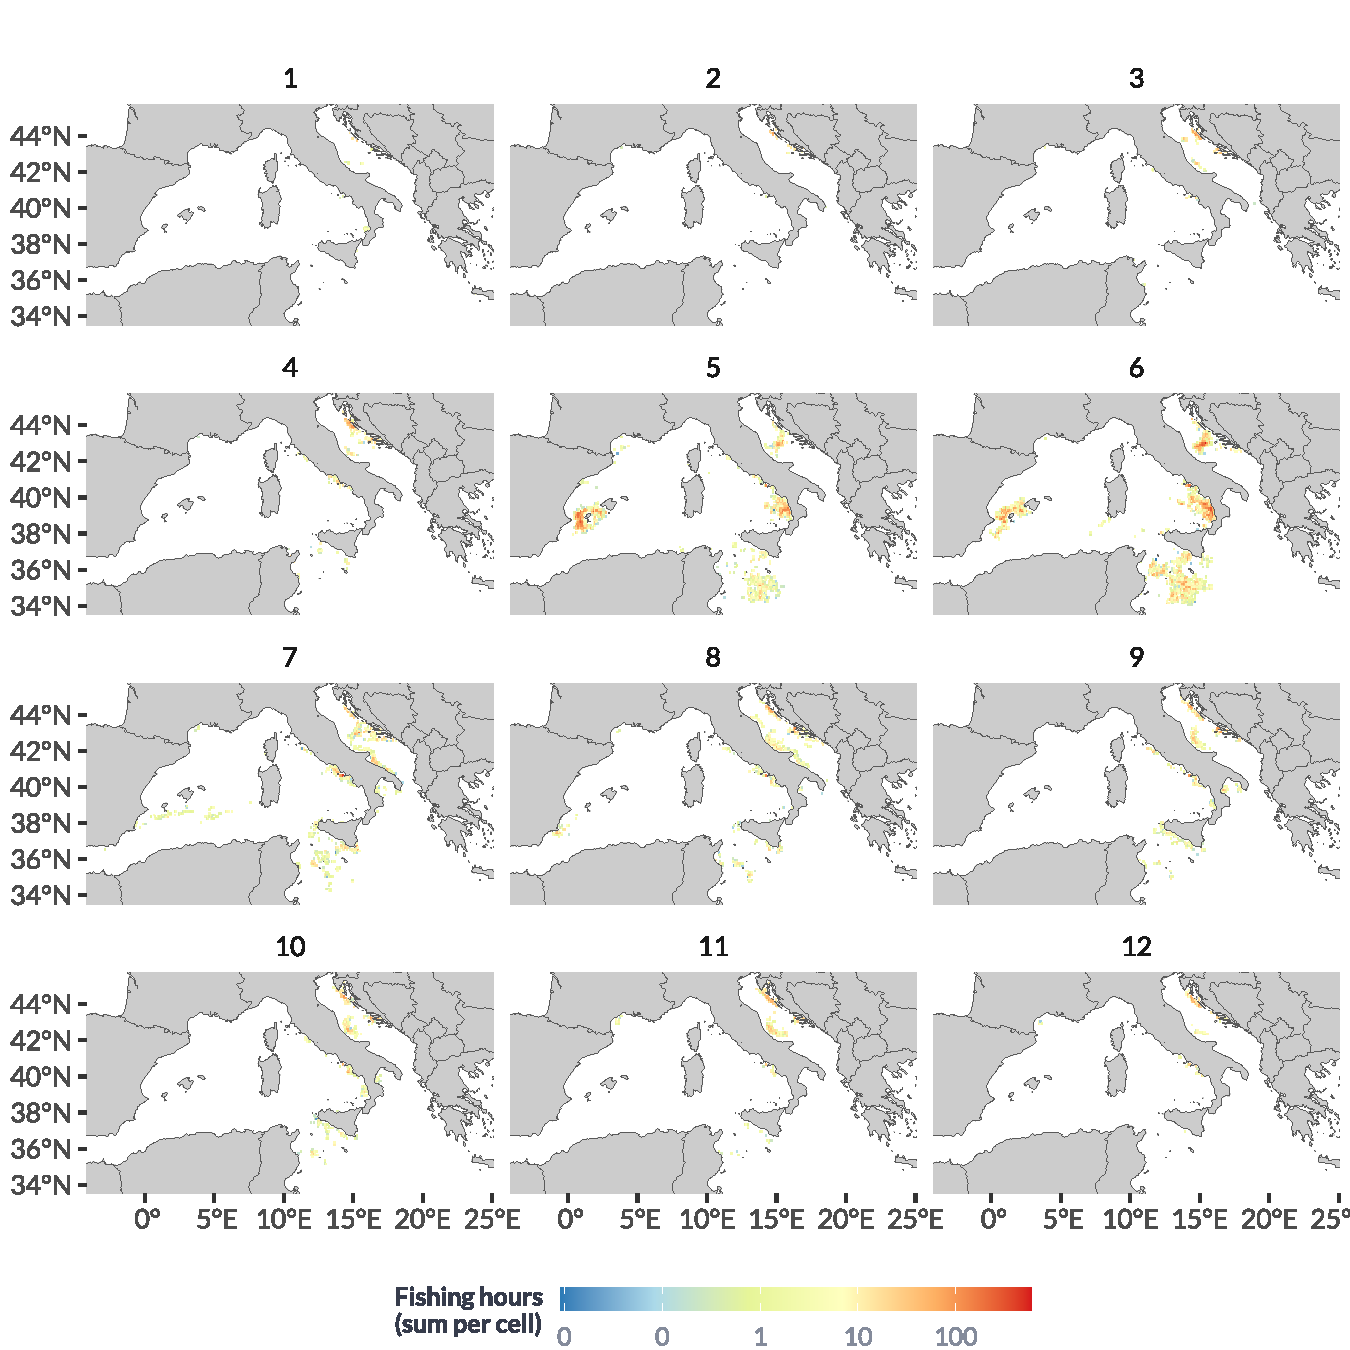
\includegraphics[width=1\linewidth, trim=0 0 0 0,clip]{Figures/plots/pss_monthly.pdf}
%	\caption{Sum of purse seine fishing hours per cell for each month between 2015-2024. Colours are on a log-scale.}
%	\label{fig:pss_monthly}
%\end{figure}

%\begin{figure}[H]
%	\centering
%	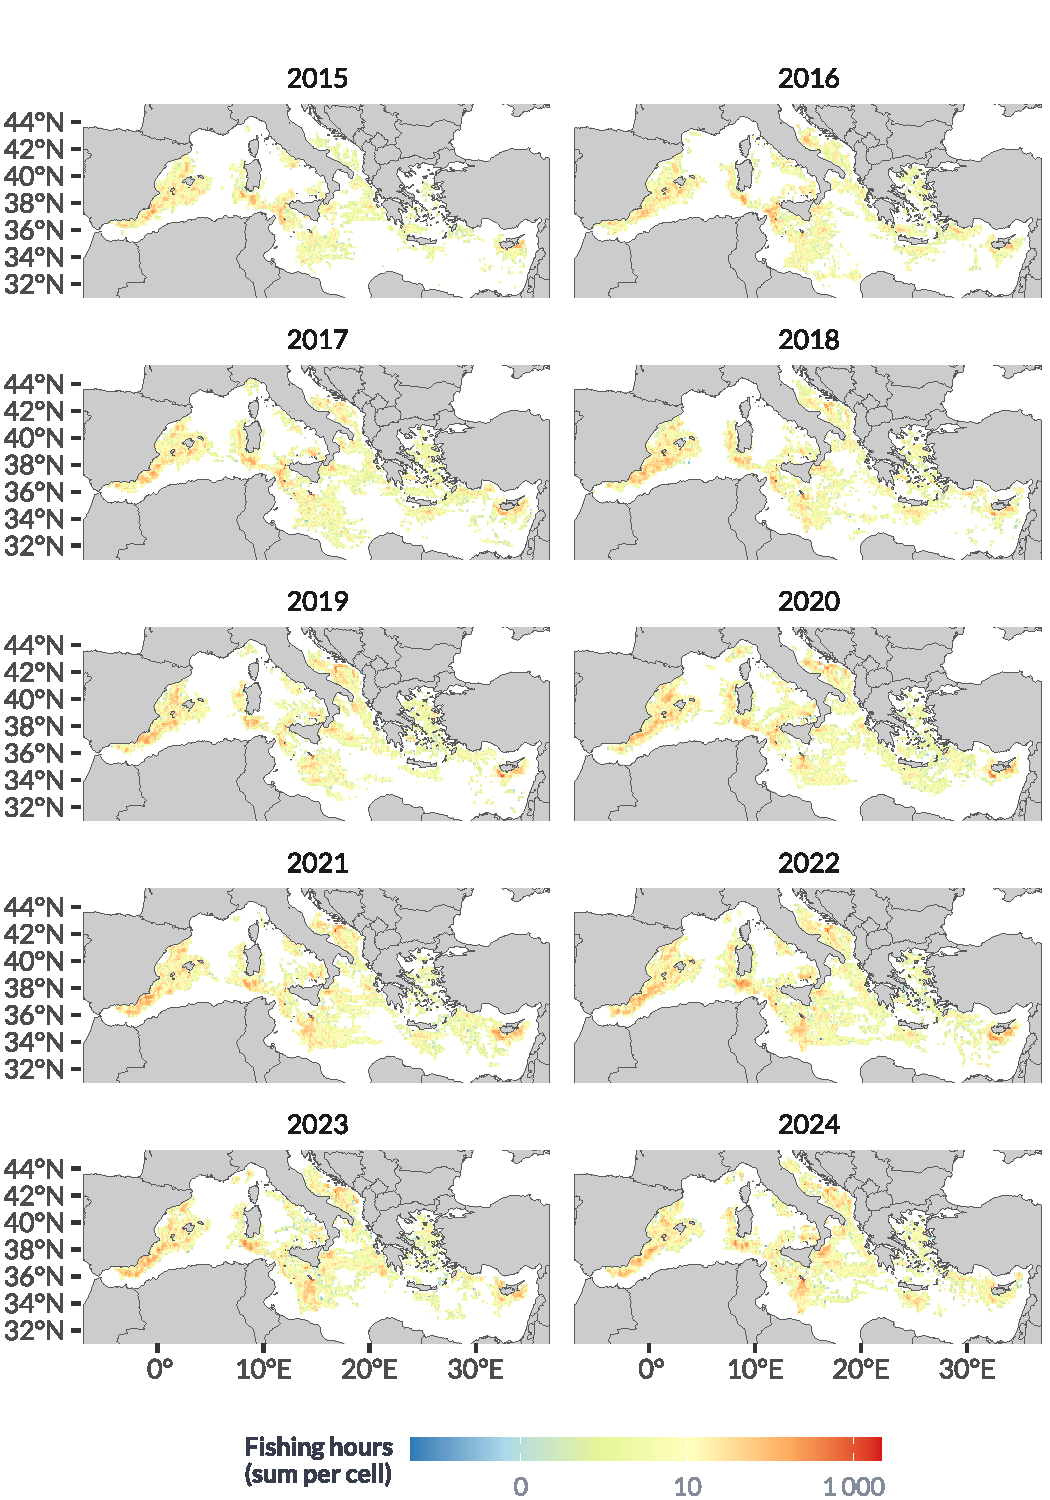
\includegraphics[width=1\linewidth, trim=0 0 0 0,clip]{Figures/plots/dll_yearly.pdf}
%	\caption{Sum of longline fishing hours per cell for each year. Colours are on a log-scale.}
%	\label{fig:dll_yearly}
%\end{figure}

%\begin{figure}[H]
%	\centering
%	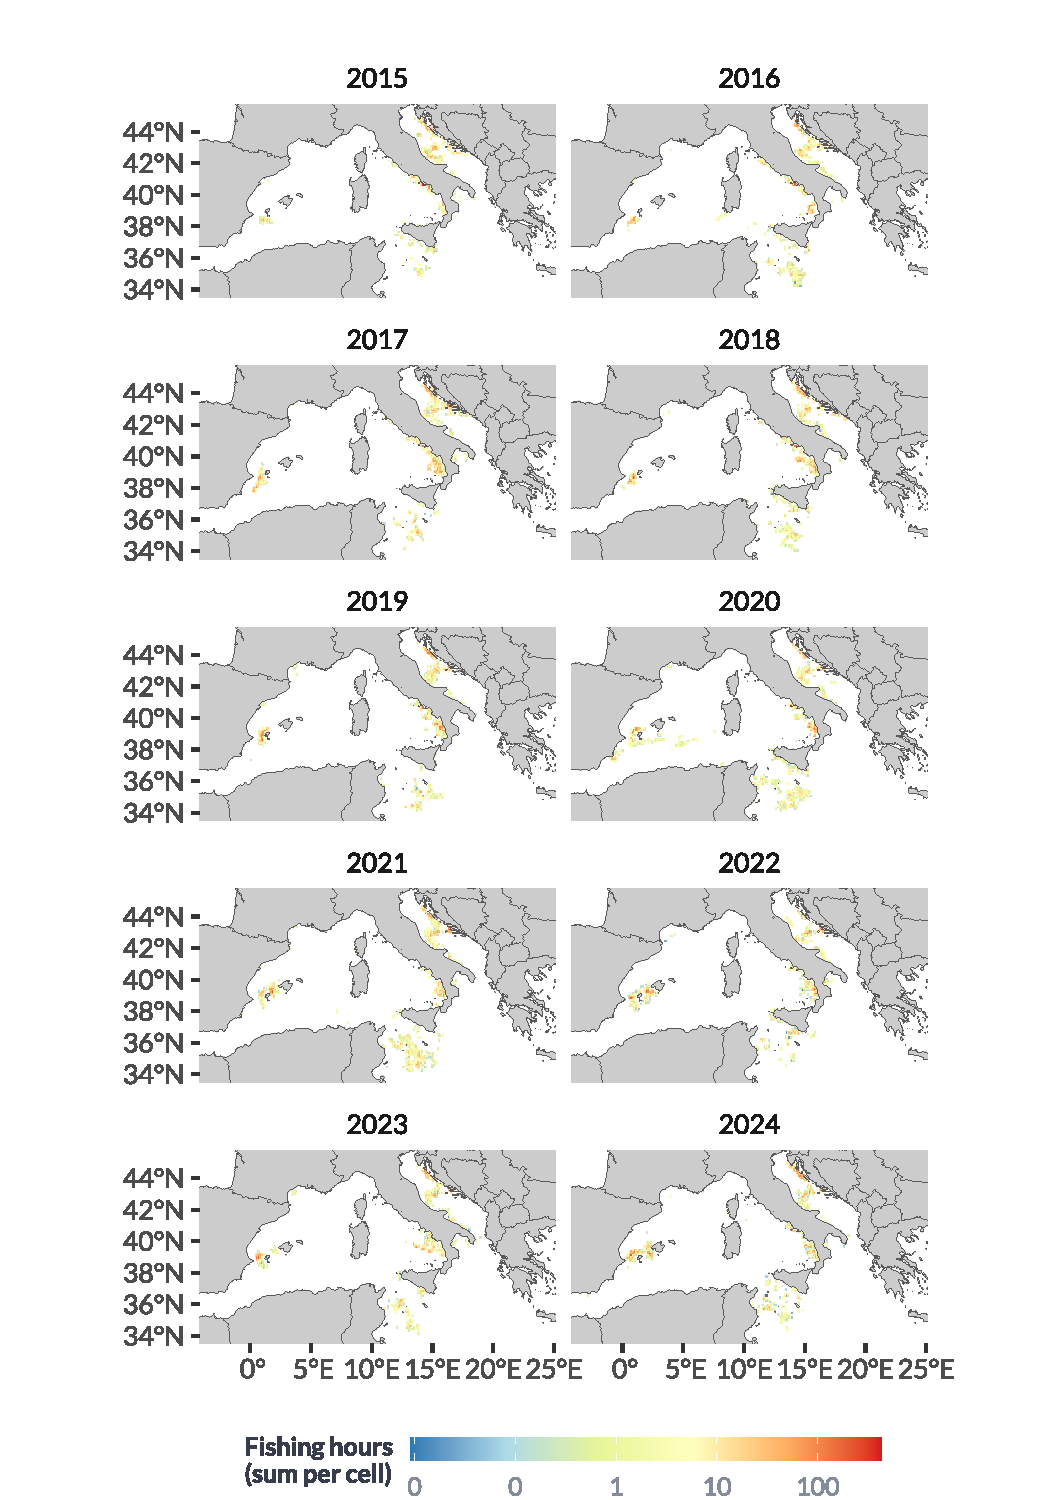
\includegraphics[width=1\linewidth, trim=0 0 0 0,clip]{Figures/plots/pss_yearly.pdf}
%	\caption{Sum of purse seine fishing hours per cell for each year. Colours are on a log-scale.}
%	\label{fig:pss_yearly}
%\end{figure}